\documentclass[border=10pt]{standalone}
\usepackage{tikz}\usepackage{amsmath}\usetikzlibrary{arrows.meta}
\begin{document}
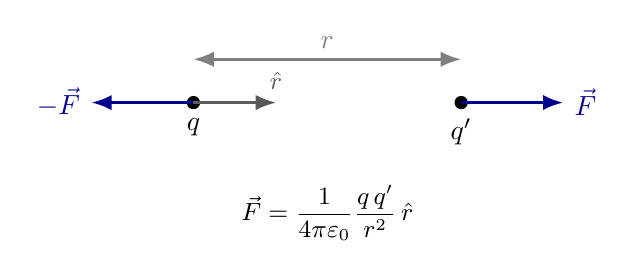
\begin{tikzpicture}[line width=0.9pt,>={Latex[length=2.6mm]}]
  \fill (0,0) circle(2.4pt) node[below=2pt]{$q$};
  \fill (3.4,0) circle(2.4pt) node[below=2pt]{$q'$};
  \draw[<->,gray] (0,0.55)--(3.4,0.55) node[midway,above]{$r$};
  \draw[->,gray!70!black] (0,0)--(1.05,0) node[above=1pt]{\small$\hat r$};
  \draw[->,blue!55!black,line width=1.3pt] (3.4,0)--(4.7,0) node[right]{$\vec F$};
  \draw[->,blue!55!black,line width=1.3pt] (0,0)--(-1.3,0) node[left]{$-\vec F$};
  \node at (1.7,-1.4){\small $\displaystyle \vec F=\frac{1}{4\pi\varepsilon_0}\frac{q\,q'}{r^2}\,\hat r$};
\end{tikzpicture}
\end{document}
